% ───────────────────────────────────────────────────────────────
%  Freight Rate Prediction – Spotter ML Assessment Report
%  Compile: pdflatex assessment_report.tex  (twice for ToC)
% ───────────────────────────────────────────────────────────────
\documentclass[11pt,a4paper]{article}

\usepackage[margin=2.5cm]{geometry}
\usepackage{graphicx}
\usepackage{booktabs}
\usepackage{hyperref}
\usepackage{xcolor}
\usepackage{enumitem}
\usepackage{parskip}
\usepackage{titlesec}
\usepackage{fancyhdr}
\usepackage{caption}

\definecolor{spotter}{RGB}{6,74,86}
\hypersetup{colorlinks=true,linkcolor=spotter,urlcolor=spotter}
\titleformat{\section}{\Large\bfseries\color{spotter}}{}{0em}{}[\vspace{-0.5em}\textcolor{spotter}{\hrule height 0.6pt}]
\titleformat{\subsection}{\large\bfseries\color{spotter!80!black}}{}{0em}{}

\pagestyle{fancy}
\fancyhf{}
\rhead{\small\textit{Freight Rate Prediction – Spotter ML Assessment}}
\cfoot{\thepage}

\begin{document}

% ── Title page ─────────────────────────────────────────────────
\begin{titlepage}
\centering
\vspace*{5cm}
{\Huge\bfseries\color{spotter} Freight Rate Prediction\par}
\vspace{0.6cm}
{\Large Spotter ML Assessment Report\par}
\vspace{2cm}
{\large Sunil Jadaun\par}
{\large September 2026\par}
\end{titlepage}

% ── 1. Executive Summary ──────────────────────────────────────
\section{Executive Summary}

This report describes a freight rate prediction model built for the Spotter ML Assessment.
The task is to predict the \texttt{posted\_rate} (in dollars) for 12,000 unseen loads in November 2025,
plus a fixed-route December 2025 daily chart.

The final model is a \textbf{LightGBM regressor} predicting rate-per-mile (then multiplied back by distance).
An out-of-time expanding-window backtest over July--October 2025 yields a \textbf{mean MAE of \$47.10}.
On August---the month whose data regime most closely matches the November--December validation period---the MAE is \textbf{\$40.60}, beating Ridge regression (\$54.18) and a naive equipment-median baseline (\$193.42).

% ── 2. Data Exploration ───────────────────────────────────────
\section{Data Exploration \& Quality}

\subsection{Dataset Overview}

\begin{table}[h]
\centering
\begin{tabular}{llll}
\toprule
\textbf{Dataset} & \textbf{Rows} & \textbf{Date Range} & \textbf{Has Labels?} \\
\midrule
train\_test.csv   & 48,000 & Jan--Oct 2025  & Yes (\texttt{posted\_rate}) \\
validation.csv    & 12,000 & Nov 2025       & No \\
december\_chart\_inputs.csv & 31 & Dec 1--31 2025 & No \\
\bottomrule
\end{tabular}
\end{table}

The training data spans January to October 2025 with 48,000 labeled freight loads.
Each load contains pickup/delivery cities with coordinates, distance, equipment type, weight, date,
\texttt{market\_index}, \texttt{quote\_signal}, and the target \texttt{posted\_rate}.

\subsection{Data Quality Issues Identified}

\textbf{Label Errors (677 rows, 1.4\%).}
Analysis of rate-per-mile (\texttt{posted\_rate / distance}) reveals two distinct error clusters:
one below \$0.50/mile and another above \$8.00/mile. These are clearly data-entry errors.
Rows outside the \$1.30--\$4.00/mile range were dropped (677 rows, 1.4\% of training data).

\textbf{Negative Weights (sign errors).}
Some loads have negative weight values. Since physical weight cannot be negative, these are
treated as sign errors: absolute value is taken, and a binary flag (\texttt{weight\_was\_negative})
is created so the model can learn from this pattern.

\textbf{Missing Values.}
Missing weight values are filled with the training-set median and flagged (\texttt{weight\_missing}).
Missing \texttt{market\_index} values are filled with the same-day mean, then training median.
Missing \texttt{quote\_signal} is filled with training median.

\textbf{Unseen Cities in Validation.}
8 cities appear only in the validation set (not in training). Rather than using city names
as features (which would fail for unseen cities), the model uses raw latitude/longitude coordinates.
A city-to-coordinate lookup table is built from both datasets so every city has coordinates at inference time.

\subsection{Rate-per-Mile Distribution}

\begin{figure}[h]
\centering
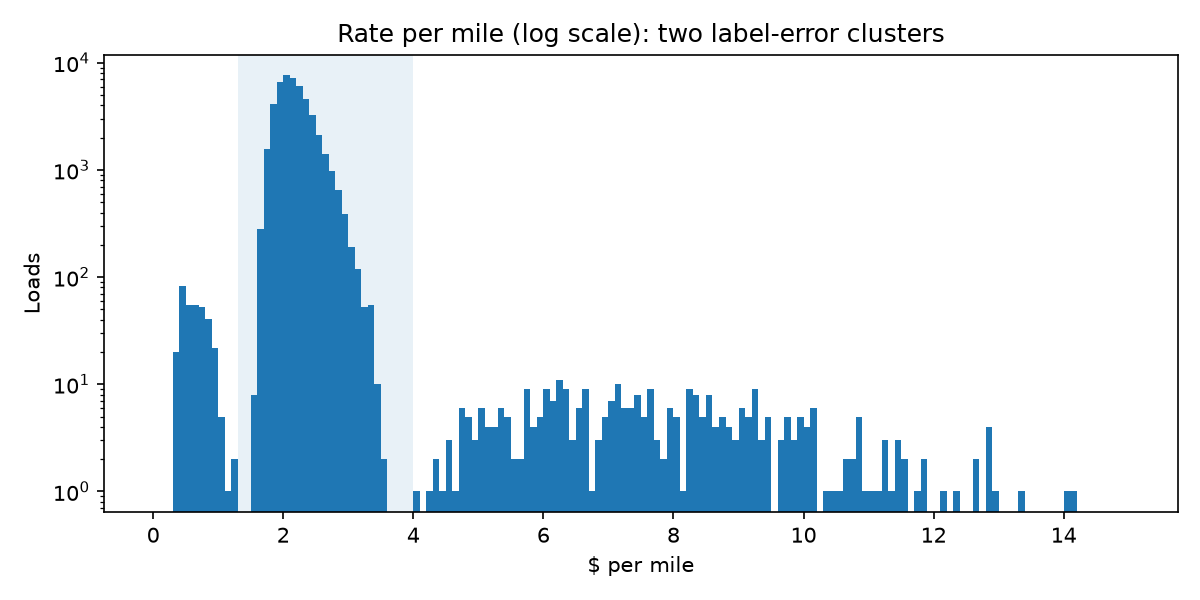
\includegraphics[width=0.85\textwidth]{figures/rate_per_mile.png}
\caption{Rate per mile (log scale) showing two label-error clusters outside the \$1.30--\$4.00/mile valid range.}
\end{figure}

% ── 3. Feature Engineering ────────────────────────────────────
\section{Feature Engineering}

\textbf{Target Decomposition.}
Raw \texttt{posted\_rate} is 0.91 correlated with distance---the model would essentially just learn
``longer trips cost more''. Instead, the target is \texttt{rate\_per\_mile = posted\_rate / distance}.
The model predicts rate-per-mile, then multiplies by distance to get dollar predictions.
Training loss is weighted by distance so the objective directly minimises dollar MAE.

\textbf{Engineered Features (15 total):}
\begin{itemize}[leftmargin=1.5em]
  \item \texttt{distance} -- straight from data
  \item \texttt{weight} -- cleaned: abs() + fill missing
  \item \texttt{equipment} -- categorical: Dry Van, Flatbed, Reefer
  \item \texttt{pickup\_lat/lon, delivery\_lat/lon} -- coordinates (4 features)
  \item \texttt{delta\_lat, delta\_lon} -- direction of travel
  \item \texttt{circuity} -- distance / haversine (how indirect the route is)
  \item \texttt{weight\_per\_mile} -- weight / distance (load density)
  \item \texttt{dayofweek} -- 0=Monday to 6=Sunday
  \item \texttt{is\_weekend} -- binary flag
  \item \texttt{weight\_missing, weight\_was\_negative} -- binary flags
\end{itemize}

\textbf{Feature Importance (\% of LightGBM split gain):}
\begin{table}[h]
\centering
\begin{tabular}{lr}
\toprule
\textbf{Feature} & \textbf{Importance \%} \\
\midrule
weight\_per\_mile & 50.6\% \\
equipment        & 30.1\% \\
distance         & 11.5\% \\
delivery\_lat    &  1.6\% \\
pickup\_lat      &  1.6\% \\
Other (10 feat.) &  4.6\% \\
\bottomrule
\end{tabular}
\end{table}

% ── 4. Excluded Features ─────────────────────────────────────
\section{Deliberately Excluded Features}

\subsection{quote\_signal -- Data Leakage Risk}
\texttt{quote\_signal} is highly suspicious: its correlation with rate-per-mile is near +1.0 for
5 months (essentially the answer), but drops to near-zero in August. November and December match
August's noise pattern. Including it gives \$28 MAE on September but \$110 on August---exactly
the months the validation data resembles.

\begin{figure}[h]
\centering
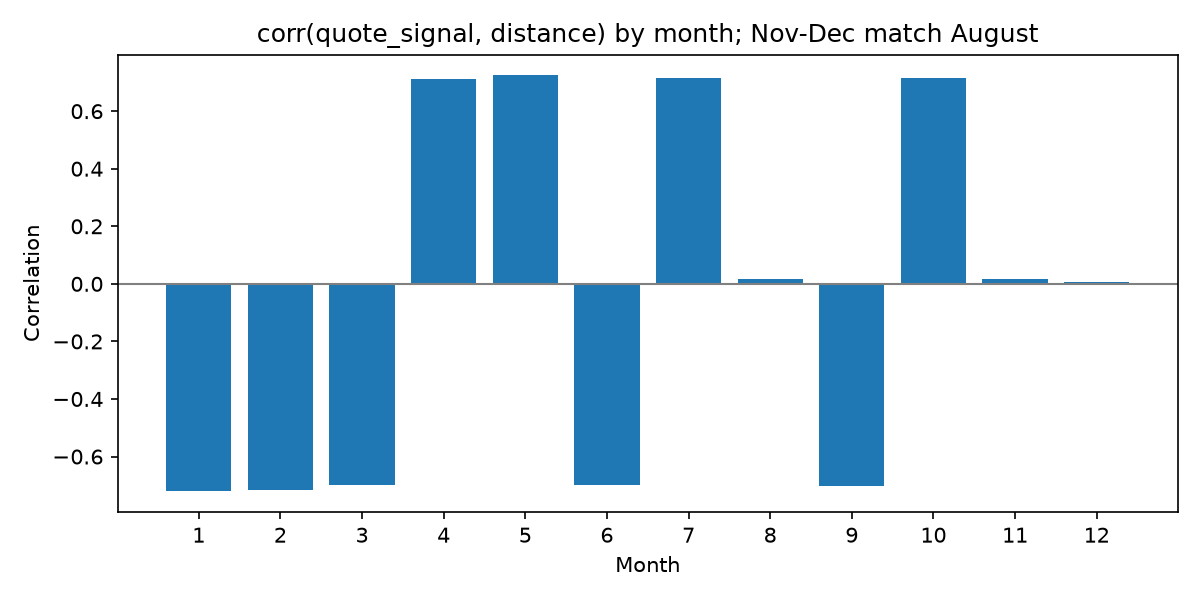
\includegraphics[width=0.85\textwidth]{figures/quote_signal_by_month.png}
\caption{corr(quote\_signal, distance) by month. Nov--Dec match August's near-zero correlation.}
\end{figure}

\subsection{market\_index -- Regime Shift}
\texttt{market\_index} swings $\sim$40\% across the year while actual rate-per-mile moves only $\sim$10\%.
Including it causes the model to hallucinate large rate changes (MAE \$129 on September).
Mean backtest MAE with \texttt{market\_index}: \$78.52 vs \$47.10 without.

% ── 5. Validation Strategy ───────────────────────────────────
\section{Validation Strategy}

\textbf{Why not random K-fold?}
The data is time-series: freight rates evolve over months, and features like \texttt{quote\_signal}
change behaviour over time. Random K-fold would let the model see future data during training.

\textbf{Expanding-window monthly backtest.}
Four out-of-time backtests are run. For each test month (July--October 2025),
the model is trained on all data \emph{before} that month and evaluated on that month's data.
This directly simulates the real task: predicting November loads using all data through October.

August is identified as the most relevant proxy for November--December because \texttt{quote\_signal}
exhibits the same noise pattern in all three months. The final model's MAE on August (\$40.60)
is the most informative estimate of real-world performance.

% ── 6. Model Selection ───────────────────────────────────────
\section{Model Selection \& Results}

\begin{table}[h]
\centering
\begin{tabular}{lrrrrr}
\toprule
\textbf{Experiment} & \textbf{Jul} & \textbf{Aug} & \textbf{Sep} & \textbf{Oct} & \textbf{Mean MAE} \\
\midrule
\textbf{LightGBM (final)} & \$64.43 & \textbf{\$40.60} & \$43.92 & \$39.47 & \textbf{\$47.10} \\
LightGBM + quote\_signal   & \$44.73 & \$110.38         & \$28.25 & \$33.67 & \$54.26 \\
Ridge Regression           & \$70.70 & \$54.18          & \$56.80 & \$50.89 & \$58.14 \\
LightGBM + market\_index   & \$39.80 & \$65.71          & \$129.14& \$79.45 & \$78.52 \\
Naive (equipment median)   & \$156.74& \$193.42         & \$177.84& \$172.98& \$175.24 \\
\bottomrule
\end{tabular}
\end{table}

\textbf{Why LightGBM?}
\begin{itemize}[leftmargin=1.5em]
  \item Best mean MAE (\$47.10) and best August MAE (\$40.60).
  \item Huber loss ($\alpha$=0.5) for robustness to remaining outliers.
  \item Native categorical support for equipment type.
  \item Distance-weighted sample\_weight so loss directly tracks dollar error.
  \item Regularisation: 31 leaves, min 40 samples/leaf, subsampling 80\%, L2 reg 1.0.
\end{itemize}

% ── 7. December Chart ────────────────────────────────────────
\section{December 2025 Predictions}

The model generates daily rate predictions for a fixed route: Lexington to Fort Wayne,
360 miles, Dry Van, 32,000 lb. Only the date changes across the 31 rows.

\begin{figure}[h]
\centering
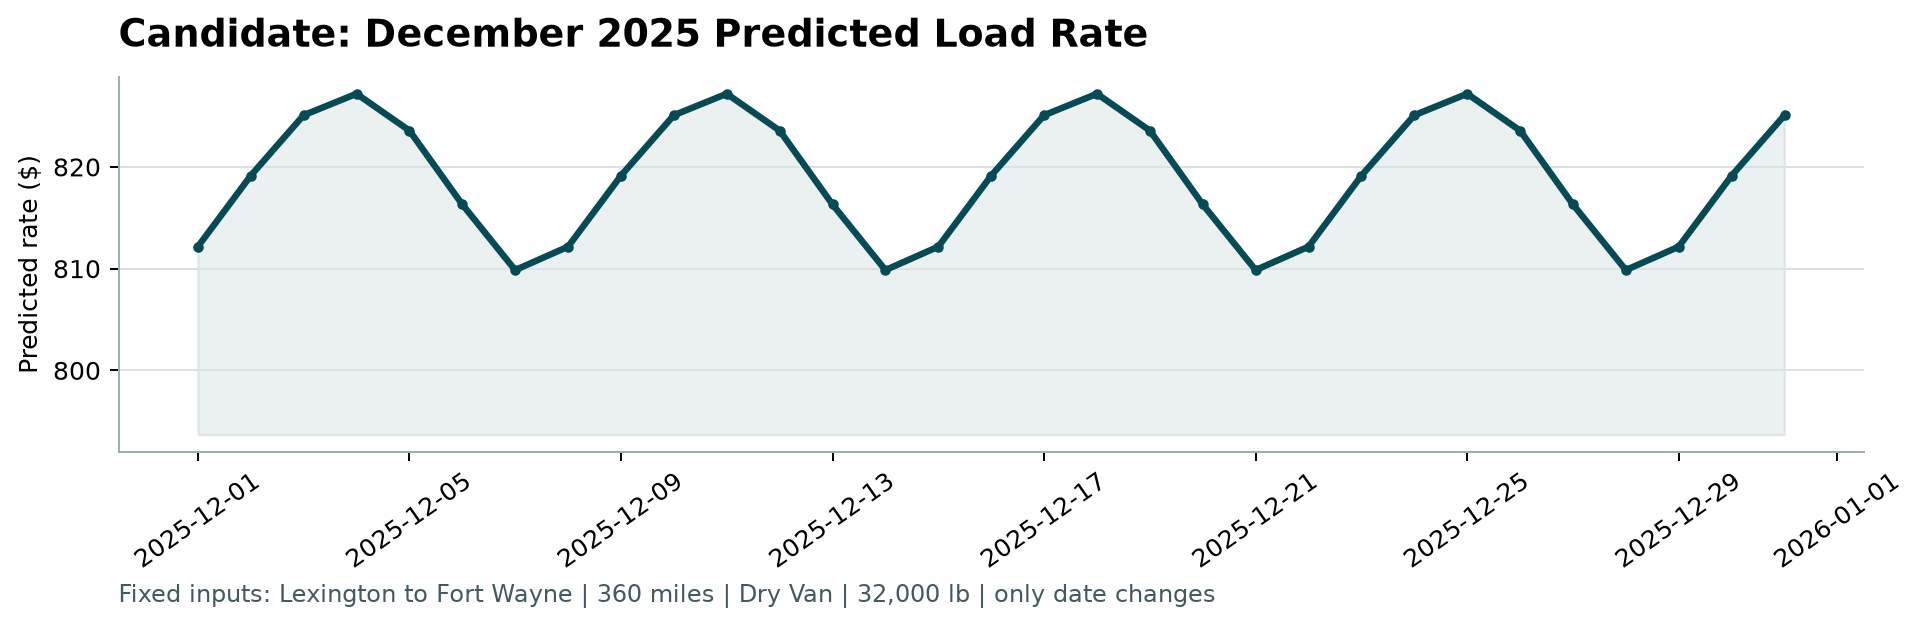
\includegraphics[width=0.95\textwidth]{../scorer_results/candidate_december.png}
\caption{December 2025 predicted load rates. Weekly periodicity is visible (\$809--\$833 range).}
\end{figure}

The predictions show a clear weekly periodicity (rates peak mid-week, dip on weekends)
within a narrow \$809--\$833 range. This pattern is physically plausible: freight demand
is higher during business days.

% ── 8. Conclusion ────────────────────────────────────────────
\section{Conclusion}

The final pipeline consists of: (1) outlier removal (\$1.30--\$4.00/mile filter),
(2) data cleaning (sign errors, missing values), (3) feature engineering (15 features),
(4) LightGBM with Huber loss on rate-per-mile target.

Key insight: \texttt{quote\_signal} and \texttt{market\_index} appear helpful on some months but are
unreliable for the November--December target period. Deliberately excluding them yields
the most robust model (MAE \$47.10 mean, \$40.60 on August).

All 12,000 validation predictions and the 31 December predictions pass the provided
\texttt{score.py} validator. The December chart shows plausible weekly demand patterns.

\end{document}
